\section{Adaptive Mesh Refinement test}
\subsection{Test 1}
There are 10720 cells: 10482 quadrilaterals, 236 pentagons, and 2 hexagons 
for a total of 43120 degrees of freedom. The distribution is given by:
\begin{figure}[H]
  \centering
  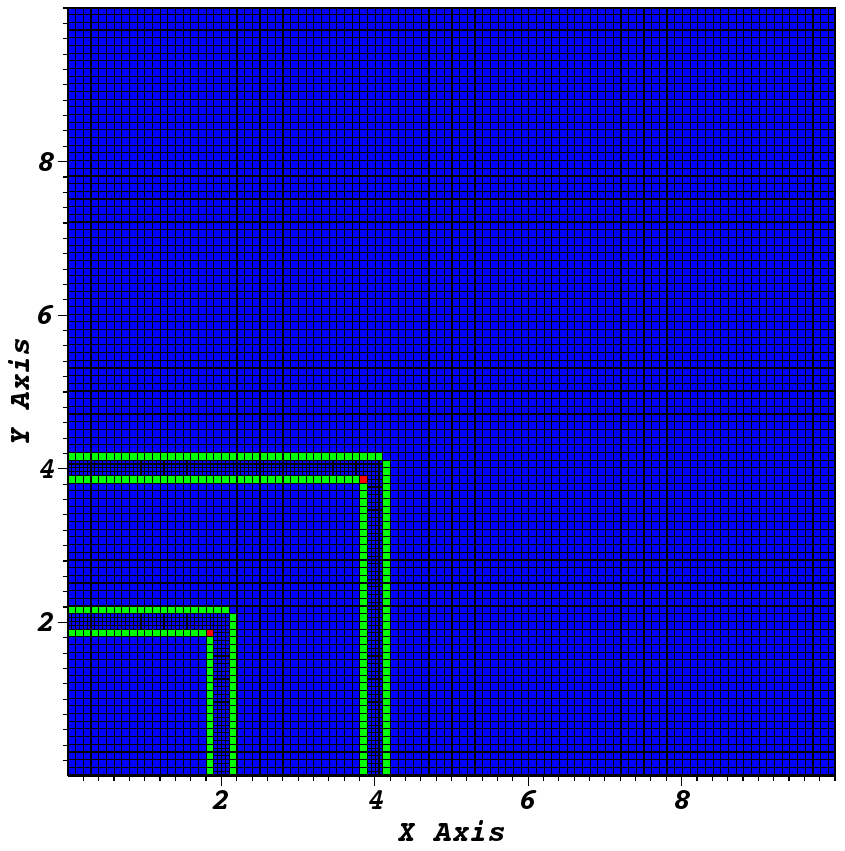
\includegraphics[width=4cm]{polygon_amr}
  \caption{Polygons distribution}
\end{figure}
\begin{itemize}
  \item Blue cells are quadrilaterals.
  \item Green cells are pentagons.
  \item Red cells are hexagons.
\end{itemize}
The domain is composed if three zones:
\begin{description}
  \item[Green zone:] $\Sigma_t=1.5cm^{-1}$, $\Sigma_s=1.44cm^{-1}$,
    source=$1cm^{-3}s^{-1}$
  \item[Red zone:] $\Sigma_t=1cm^{-1}$, $\Sigma_s=0.9cm^{-1}$, no source
  \item[Blue zone:] $\Sigma_t=1cm^{-1}$, $\Sigma_s=0.3cm^{-1}$, no source
\end{description}
We use a $S_{16}$ GLC quadrature, with SI, tolerance is $10^{-8}$, PWLD,
bottom and left boundaries are reflective, right and top boundaries vacuum.
\begin{table}[H]
  \caption{Comparison of preconditioners on AMR mesh.}
  \begin{center}
    \begin{tabular}{|c|c|c|c|c|c|c|}
      \hline
       & No-DSA & CG & PCG-SGS & PCG-MLU & PCG-MLM & AGMG \\
      \hline
      SI iter    & 184     & 19      & 19       & 19      & 19       & 19 \\
      Prec (s)   & NA      & NA      & 0.043463 & 0.358002 & 1.19301 & 0.0111\\
      MIP (s)    & NA      & 48.1908 & 81.0992  & 25.2699 & 25.0699  & 
      2.56198\\
      CG iter    & NA      & 11300   & 4734     & 361     & 361      & 264 \\
      Total (s)  & 802.985 & 138.825 & 172.423  & 116.018 & 116.517  &
      94.1963\\
      \hline
    \end{tabular}
  \end{center}
\end{table}
\begin{figure}[H]
  \centering
  \includegraphics[width=4cm]{amr_1}
  \caption{Scalar flux on AMR mesh.}
\end{figure}
\subsection{Test 2}
There are 10720 cells: 10482 quadrilaterals, 236 pentagons, and 2 hexagons 
for a total of 43120 degrees of freedom. The distribution is given by:
\begin{figure}[H]
  \centering
  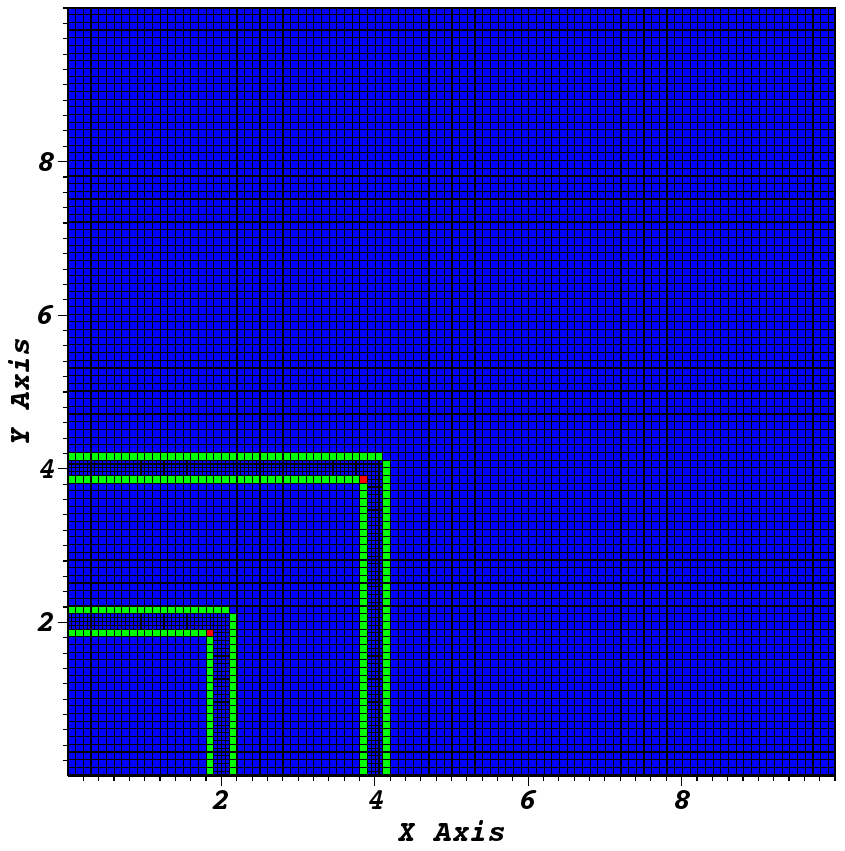
\includegraphics[width=4cm]{polygon_amr}
  \caption{Polygons distribution}
\end{figure}
\begin{itemize}
  \item Blue cells are quadrilaterals.
  \item Green cells are pentagons.
  \item Red cells are hexagons.
\end{itemize}
The domain is composed if three zones:
\begin{description}
  \item[Green zone:] $\Sigma_t=1cm^{-1}$, $\Sigma_s=0.9cm^{-1}$,
    source=$1cm^{-3}s^{-1}$
  \item[Red zone:] $\Sigma_t=1.5cm^{-1}$, $\Sigma_s=1.44cm^{-1}$, no source
  \item[Blue zone:] $\Sigma_t=1cm^{-1}$, $\Sigma_s=0.3cm^{-1}$, no source
\end{description}
We use a $S_{16}$ GLC quadrature, with SI, tolerance is $10^{-8}$, PWLD,
bottom and left boundaries are reflective, right and top boundaries vacuum.
\begin{table}[H]
  \caption{Comparison of preconditioners on AMR mesh.}
  \begin{center}
    \begin{tabular}{|c|c|c|c|c|c|c|}
      \hline
       & No-DSA & CG & PCG-SGS & PCG-MLU & PCG-MLM & AGMG \\
      \hline
      SI iter    & 171   & 19      & 19        & 19      & 19      & 19 \\
      Prec (s)   & NA    & NA      & 0.0176618 & 0.38593 & 1.35936 & 0.0101 \\
      MIP (s)    & NA    & 50.5863 & 89.6251   & 28.5313 & 28.7984 & 2.64447\\
      CG iter    & NA    & 11474   & 4654      & 360     & 361     & 264 \\
      Total (s)  & 736.2 & 142.471 & 189.641   & 129.449 & 131.963 & 99.9768\\
      \hline
    \end{tabular}
  \end{center}
\end{table}
\begin{figure}[H]
  \centering
  \includegraphics[width=4cm]{amr_2}
  \caption{Scalar flux on AMR mesh.}
\end{figure}
